\documentclass{zkdl-presentation-template}

\title[NNT. PlonK]{\textbf{Number Theoretic Transform (NTT)}}
\author{Distributed Lab}
\date{January 21, 2025}
\homepage{zkdl-camp.github.io}
\github{ZKDL-Camp}

\begin{document}
    \frame {
        \tikz [remember picture,overlay]
        \node at
        ([yshift=1.5cm,xshift=-1.5cm]current page.south east)
    %or: (current page.center)
            {
\includegraphics[width=60pt]{images/logo.png}};

        \titlepage
    }

    \begin{frame}{Plan}
        \tableofcontents
    \end{frame}

    \section{Recap on Interpolation}

    \subsection{Polynomial Interpolation is a Universal Encoder}
    \begin{frame}{Polynomial Interpolation}
        \begin{block}{Notice}
            All the previous protocols use the idea that polynomials 
            are \textbf{universal data encoders}. We can encode any 
            set of scalars $(a_0,\dots,a_{N-1}) \in \mathbb{F}^N$ 
            using \textbf{interpolation}:
            \begin{equation*}
                p(x_j) = a_j, \quad j = 0,\dots,N-1, \quad \text{$\{x_j\}_{j \in [N]}$ are fixed}
            \end{equation*}
        \end{block}

        \begin{figure}
            \centering
            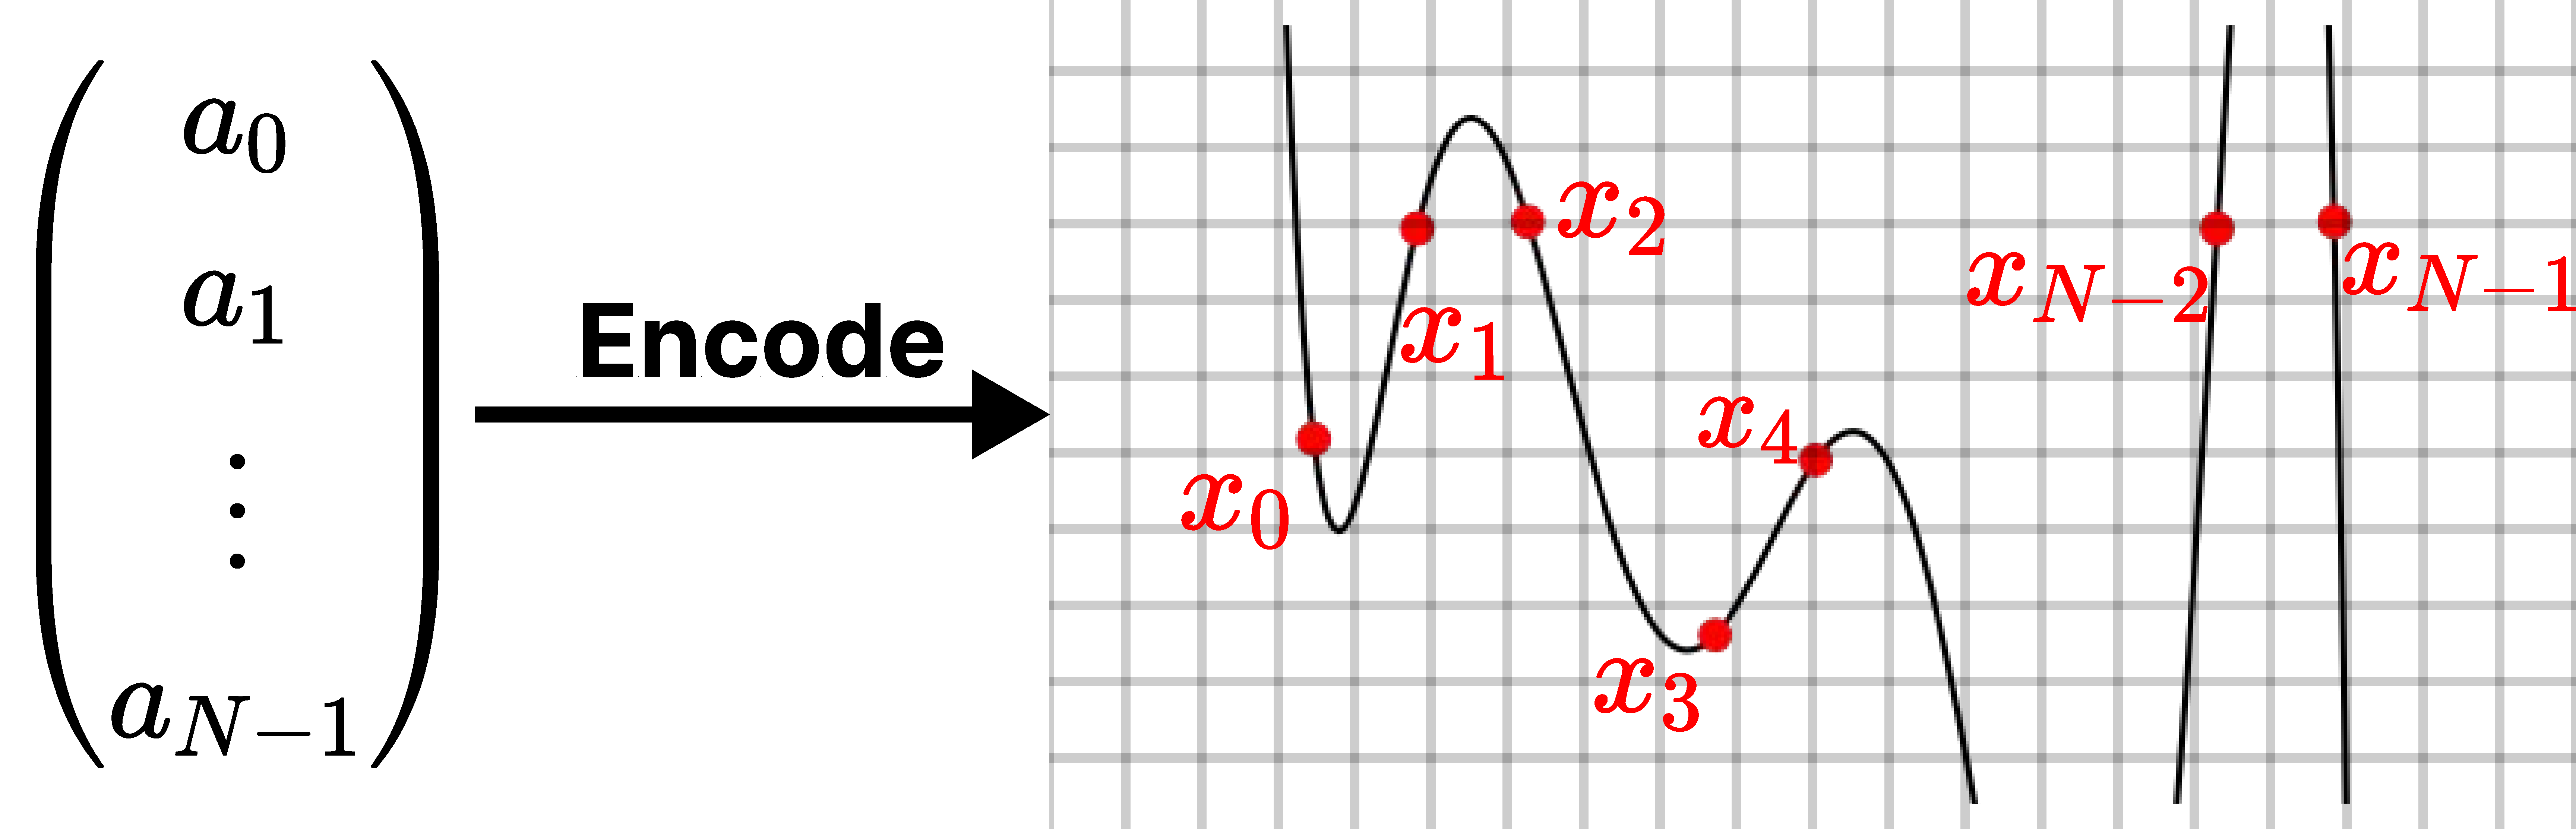
\includegraphics[width=\textwidth]{images/lecture_13/encoding.pdf}
            \caption{Polynomial Interpolation as a universal encoder.}
        \end{figure}        
    \end{frame}

    \begin{frame}{Polynomial Interpolation}
        \begin{example}
            In Groth16, we used interpolation of $3n$ polynomials:
            \begin{equation*}
                L_j(i) = \ell_{i,j}, \quad R_j(i) = r_{i,j}, \quad O_j(i) = o_{i,j},
            \end{equation*}
            where $\ell_{i,j}, r_{i,j}, o_{i,j}$ are the elements of constraint
            matrices $L, R, O$ (left, right, and output).
        \end{example}

        \begin{columns}
            % Description
            \begin{column}{0.65\textwidth}
                However, in PlonK we have witnessed $a(\omega^j) = A_j$ where
                $A_j$ are the elements of the left trace vector $A$.

                \begin{alertblock}{Question}
                    What the heck is this $\omega$? Why do we 
                    need it? How it helps?
                \end{alertblock}
            \end{column}
            % Column 2    
            \begin{column}{0.35\textwidth}
                \begin{figure}
                    \centering
                    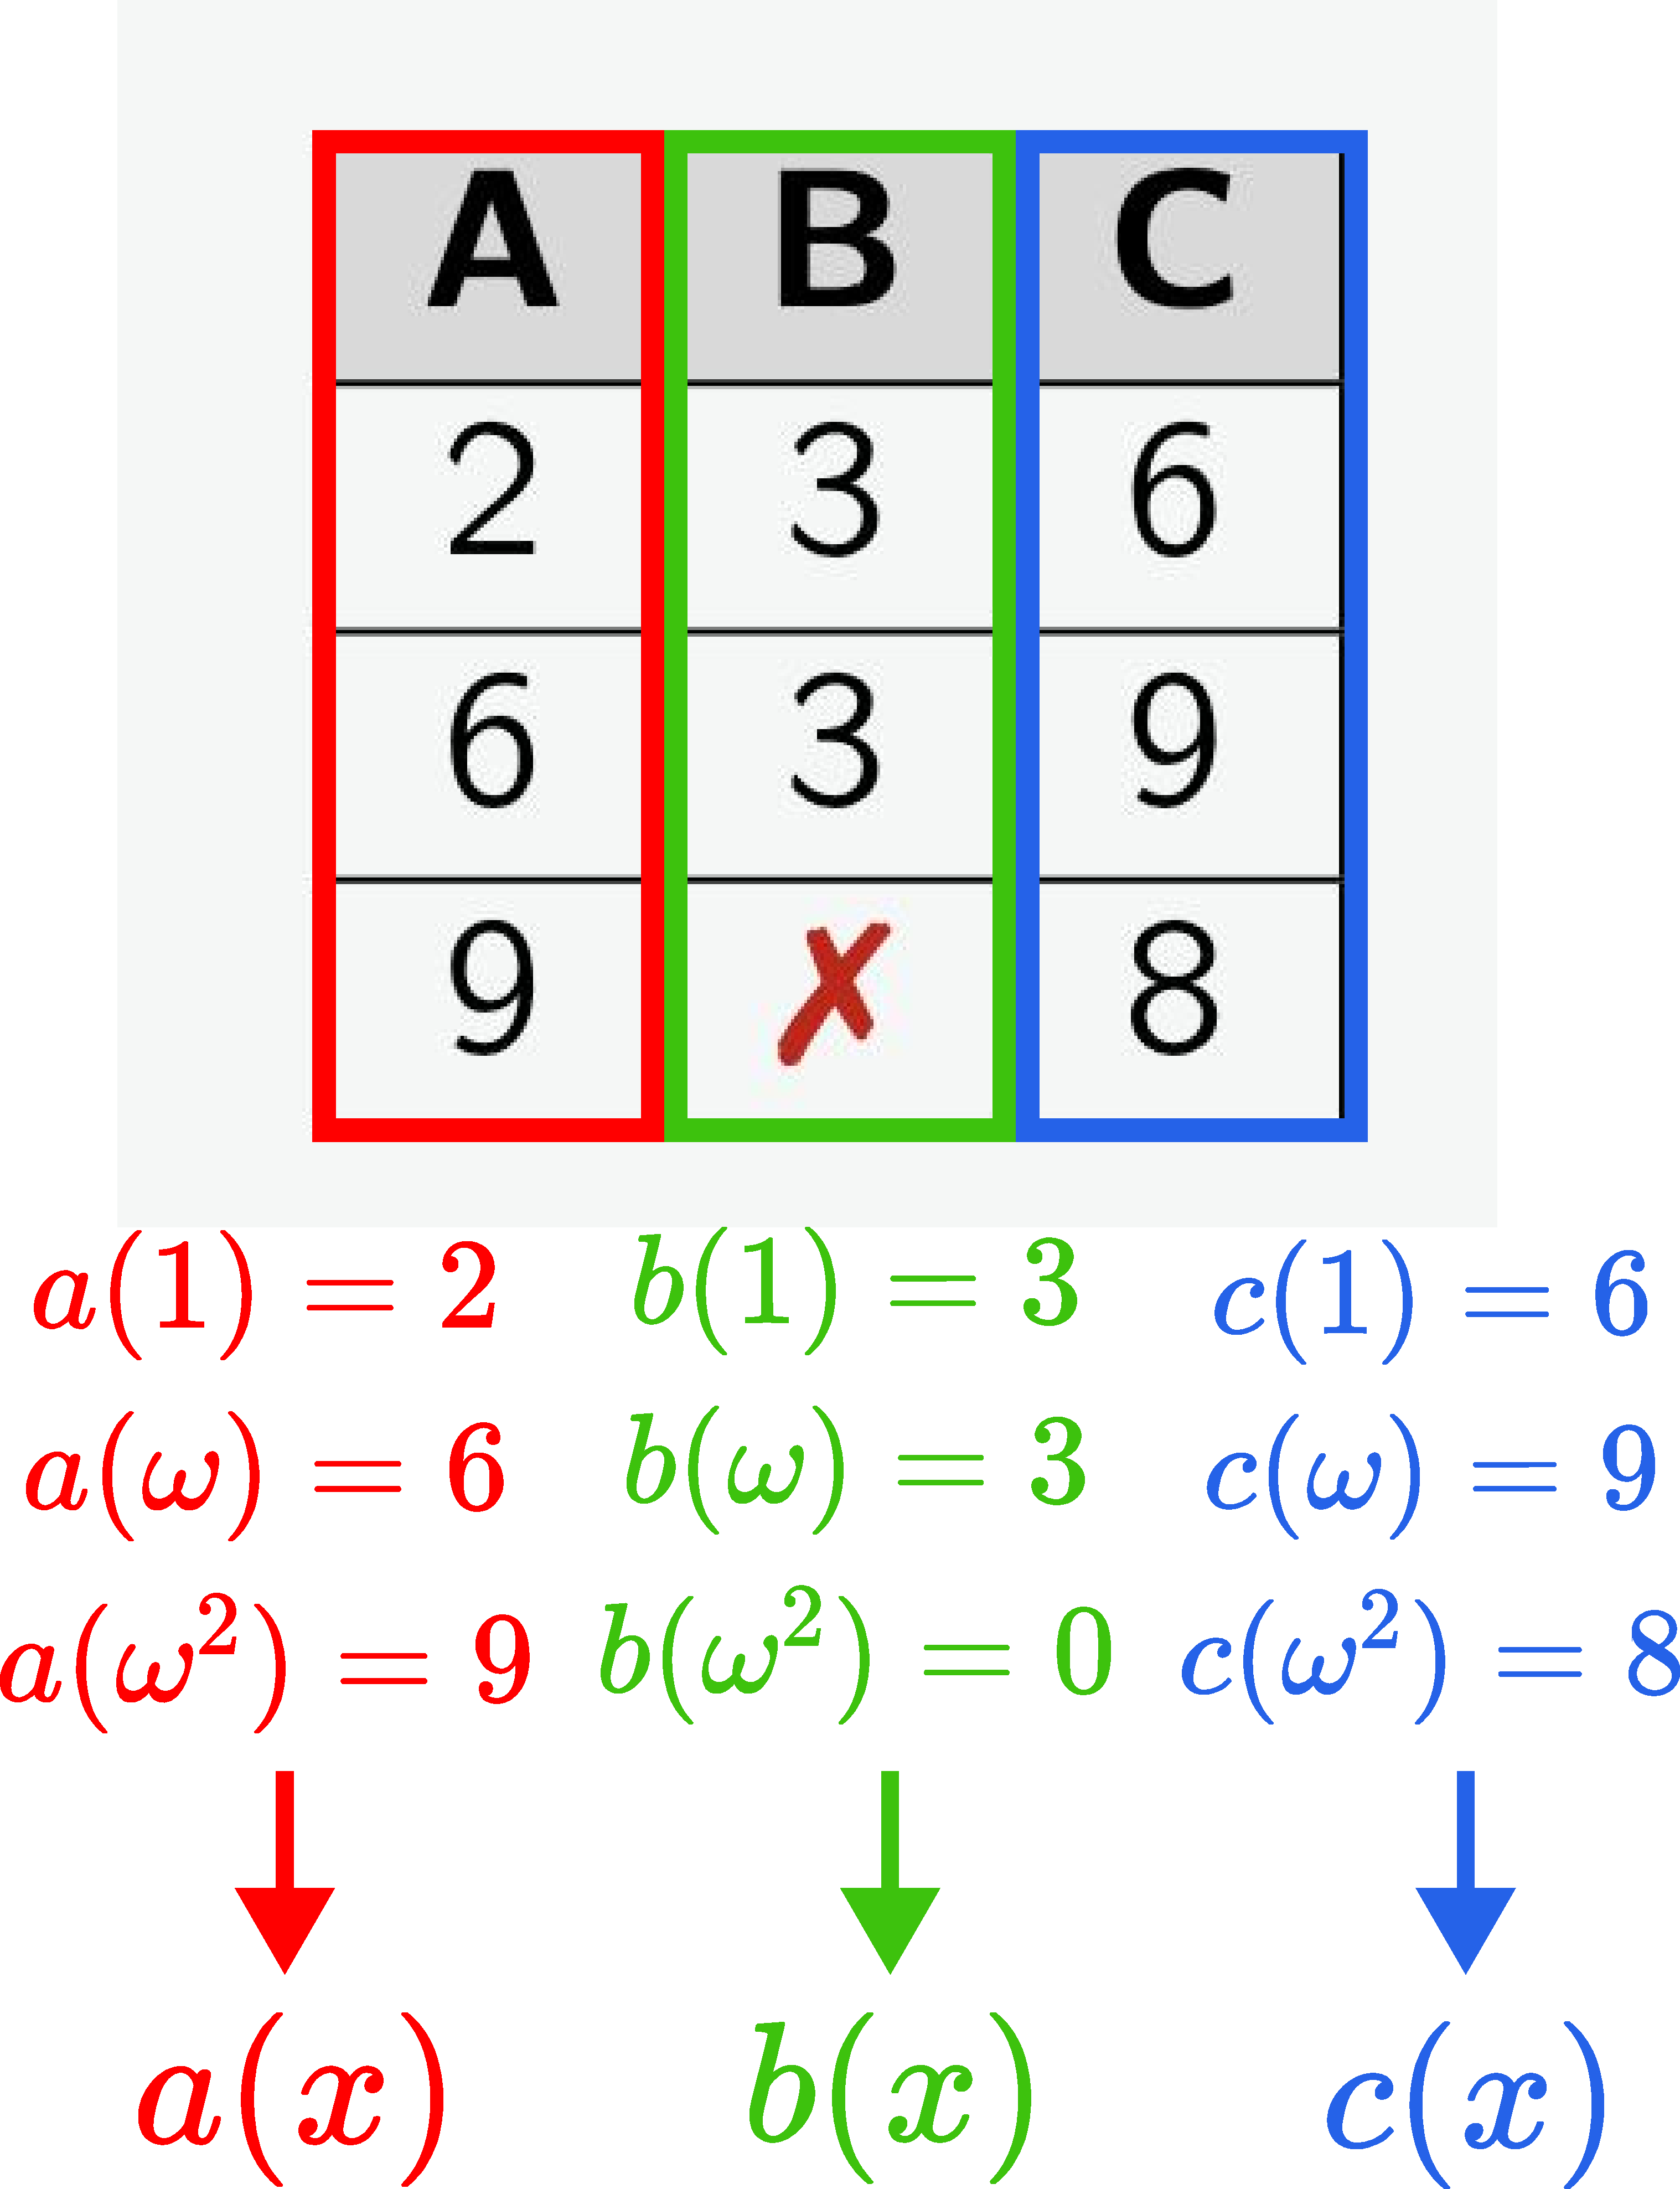
\includegraphics[width=0.8\textwidth]{images/lecture_13/plonk_table.pdf}
                \end{figure}
            \end{column}
        \end{columns}
    \end{frame}

    \subsection{Motivation for NTT}
    \begin{frame}{Why we need something advanced?}
        \begin{block}{Recall}
            The interpolation formula in given by:
            \begin{equation*}
                p(x) = \sum_{i=0}^{N-1} a_i \cdot \ell_i(x), \quad \ell_i(x) = \prod_{j=0, j \neq i}^{N-1} \frac{x - x_j}{x_i - x_j}
            \end{equation*}
        \end{block}

        \begin{alertblock}{Question}
            What is the naive complexity of this interpolation implementation?
        \end{alertblock}

        \begin{block}{Observation}
            Through careful choice of $\{x_j\}_{j \in [N]}$, we can reduce the
            complexity of interpolation, multiplication, or other complex
            operations to $\mathcal{O}(N \log N)$. \textbf{Spoiler:} we will use
            the $n$th roots of unity domain $\Omega = \{\omega^j\}_{j \in [N]}$.
            Let us see why it helps.
        \end{block}
    \end{frame}

    \section{Roots of Unity}
    \subsection{Multiplicative Subgroup of Finite Fields}
    \begin{frame}{Multiplicative Subgroup.}
        We know that $\mathbb{F}_p$ is a \textbf{field}: we have a usual arithmetic $+,\times$.

        \begin{alertblock}{Question}
            Does $(\mathbb{F}_p, \times)$ form a group?
        \end{alertblock}

        No, since $0$ does not have an inverse. But, if we consider
        $(\mathbb{F}_p \setminus \{0\}, \times)$, we do have a group structure!

        \begin{definition}
            A \textbf{multiplicative group} of a finite field $\mathbb{F}$, denoted as $\mathbb{F}^{\times}$, is a multiplicative group $(\mathbb{F} \setminus \{0\}, \times)$.
        \end{definition}

        \begin{block}{Number of Elements}
            The number of elements in $\mathbb{F}^{\times}_p$ is $p - 1$. 
        \end{block}
    \end{frame}

    \begin{frame}{Primitive Root}
        \begin{theorem}
            Multiplicative group of a finite field $\mathbb{F}^{\times}_p$ is
            \textbf{cyclic}. The generators $\omega$ of this group are called
            \textbf{primitive roots}.
        \end{theorem}

        \begin{example}
            $\omega=3$ is the primitive root of $\mathbb{F}_7$. Indeed,
            \begin{align*}
                3^1 = 3, \quad 3^2 = 2, \quad 3^3 = 6, \quad 3^4 = 4, \quad 3^5 = 5, \quad 3^6 = 1.
            \end{align*} 

            Clearly, $\langle \omega \rangle = \mathbb{F}_7^{\times}$.
        \end{example}

        The set $\mathbb{F}^{\times}_p$ is not useful on its own. However, we
        can consider the following set, called \textbf{$r$-th roots of unity}:
        \begin{equation*}
            \Omega_r = \{ \omega \in \mathbb{F}^{\times}_p \mid \omega^r = 1 \} \subset \mathbb{F}_p^{\times}.
        \end{equation*}

        \vspace{-15px}

        \textcolor{purple}{\textbf{Question.}} When such cyclic group exists?
    \end{frame}

    \begin{frame}{Roots of Unity}
        \begin{theorem}[Lagrange Theorem]
            If $\mathbb{H} \leq \mathbb{G}$ is a subgroup of any finite group $\mathbb{G}$, then $\text{ord}(\mathbb{H}) \mid \text{ord}(\mathbb{G})$.
        \end{theorem}

        \begin{corollary}
            If $\Omega_r$ is a subgroup of $\mathbb{F}_p^{\times}$, then $r \mid
            (p - 1)$.
        \end{corollary}

        \begin{alertblock}{Some other Notes}
            Moreover, one might prove in the opposite direction:
            \begin{itemize}
                \item If $r \mid (p-1)$, then there exists a subgroup $\Omega_r
                \leq \mathbb{F}_p^{\times}$.
                \item Its generator is given by $\omega = g^{(p-1)/r}$ where 
                $\langle g \rangle = \mathbb{F}_p^{\times}$.
            \end{itemize} 
        \end{alertblock}

        \begin{block}{Yet another note}
            Typically, we would need $r$ to be the power of two. We will see why 
            in the NTT section.
        \end{block}
    \end{frame}

    \begin{frame}{Complex Analysis Interpretation}
        \begin{figure}
            \centering
            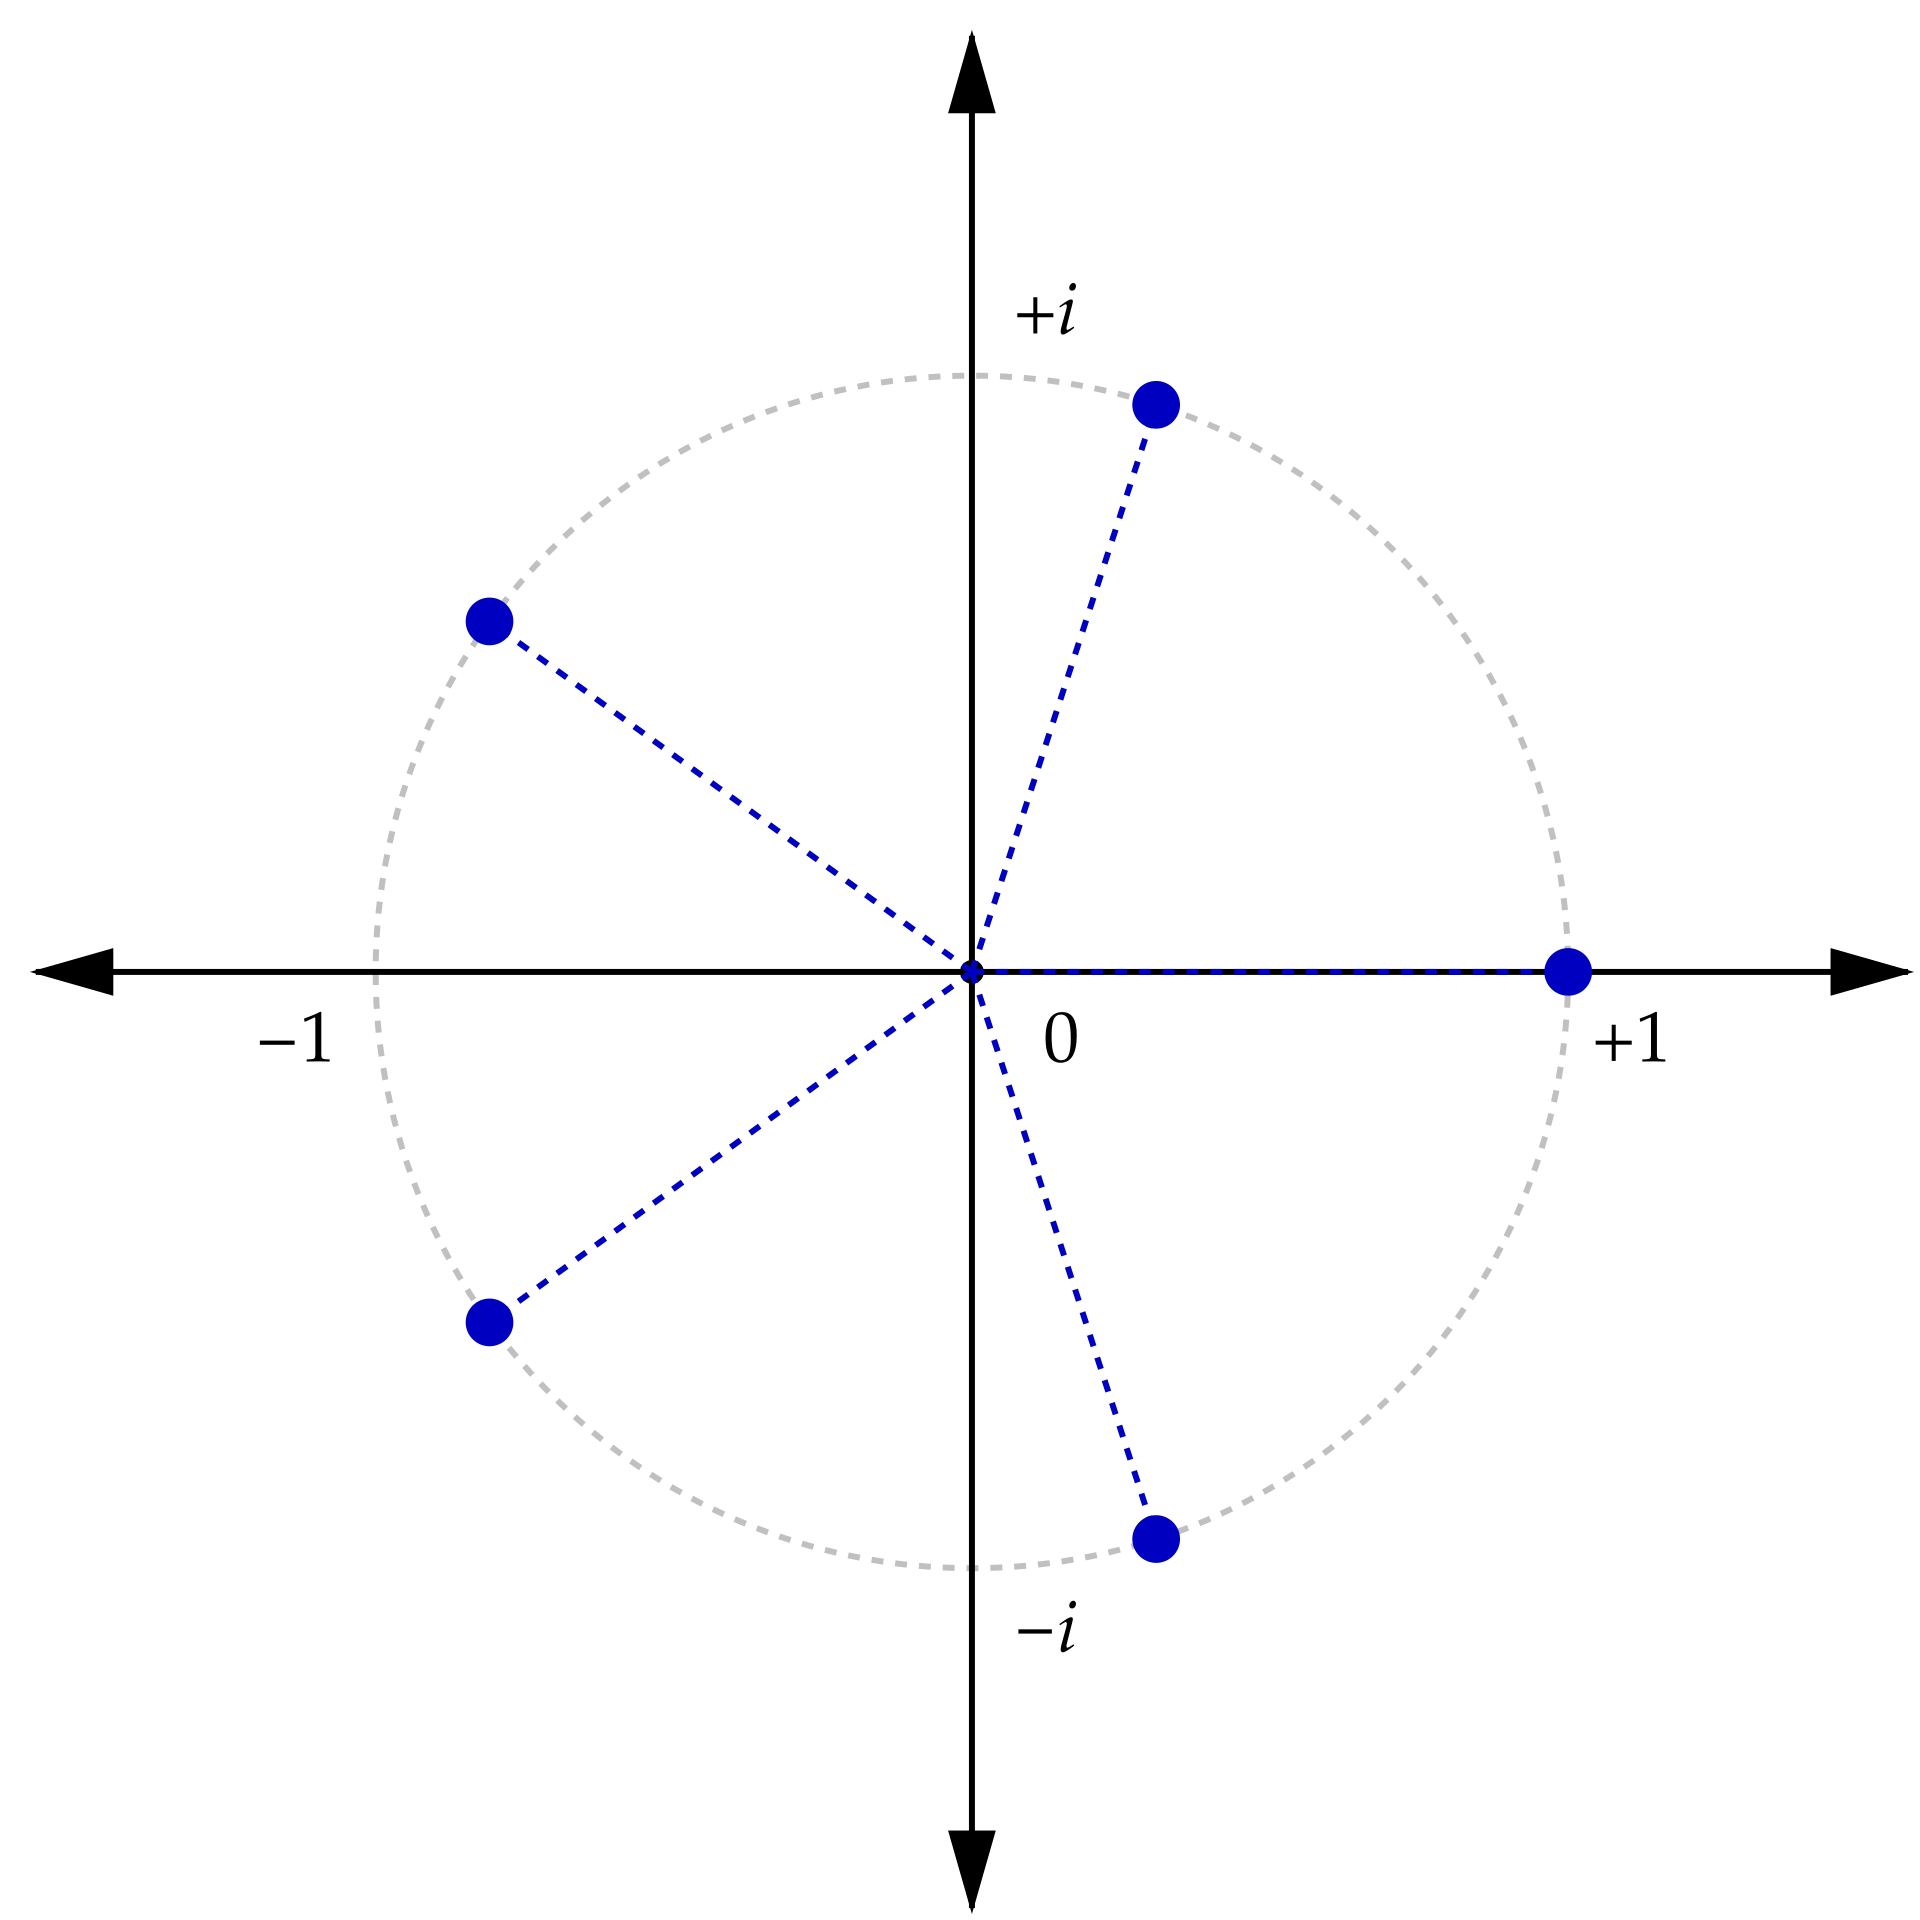
\includegraphics[width=0.5\textwidth]{images/lecture_13/roots.png}
            \caption{Visualization of the roots of unity $\Omega_5 = \{z \in \mathbb{C}: z^5=1 \}$.}
        \end{figure}

        On the complex plane, the generator of the $r$-th roots of unity
        $\Omega_r$ is given by $\zeta_r = e^{2\pi i/r}$. In a finite field,
        we do not have such a luxury.
    \end{frame}

    \subsection{Barycentric Interpolation}
    \begin{frame}{Vanishing Polynomial}
        \begin{block}{Definition}
            The \textbf{vanishing polynomial} $z_D(x)$ of a set $D \subset \mathbb{F}_p$
            is a polynomial satisfying $z_D(d) = 0$ for all $d \in D$.
        \end{block}
        Vanishing polynomials are always of form $z_D(x) = c \cdot \prod_{d \in
        D}(x-d)$. 

        The interesting question is: what is the vanishing polynomial of the
        $r$-th roots of unity $\Omega_r$? For simplicity, assume $c=1$.

        \begin{block}{Lemma}
            The vanishing polynomial of $\Omega_r$ is $z_{\Omega}(x) = x^r-1$.
        \end{block}

        \textbf{Proof Idea.} Since for any $\zeta \in \Omega_r$ we have $\zeta^r=1$, or, 
        equivalently, $\zeta^r-1$. Thus, any $\zeta \in \Omega_r$ is a root of $z_{\Omega}(x) = x^r-1$.
    \end{frame}

    \begin{frame}{Vanishing Polynomial over $\mathbb{R}$}
        \begin{figure}
            \centering
            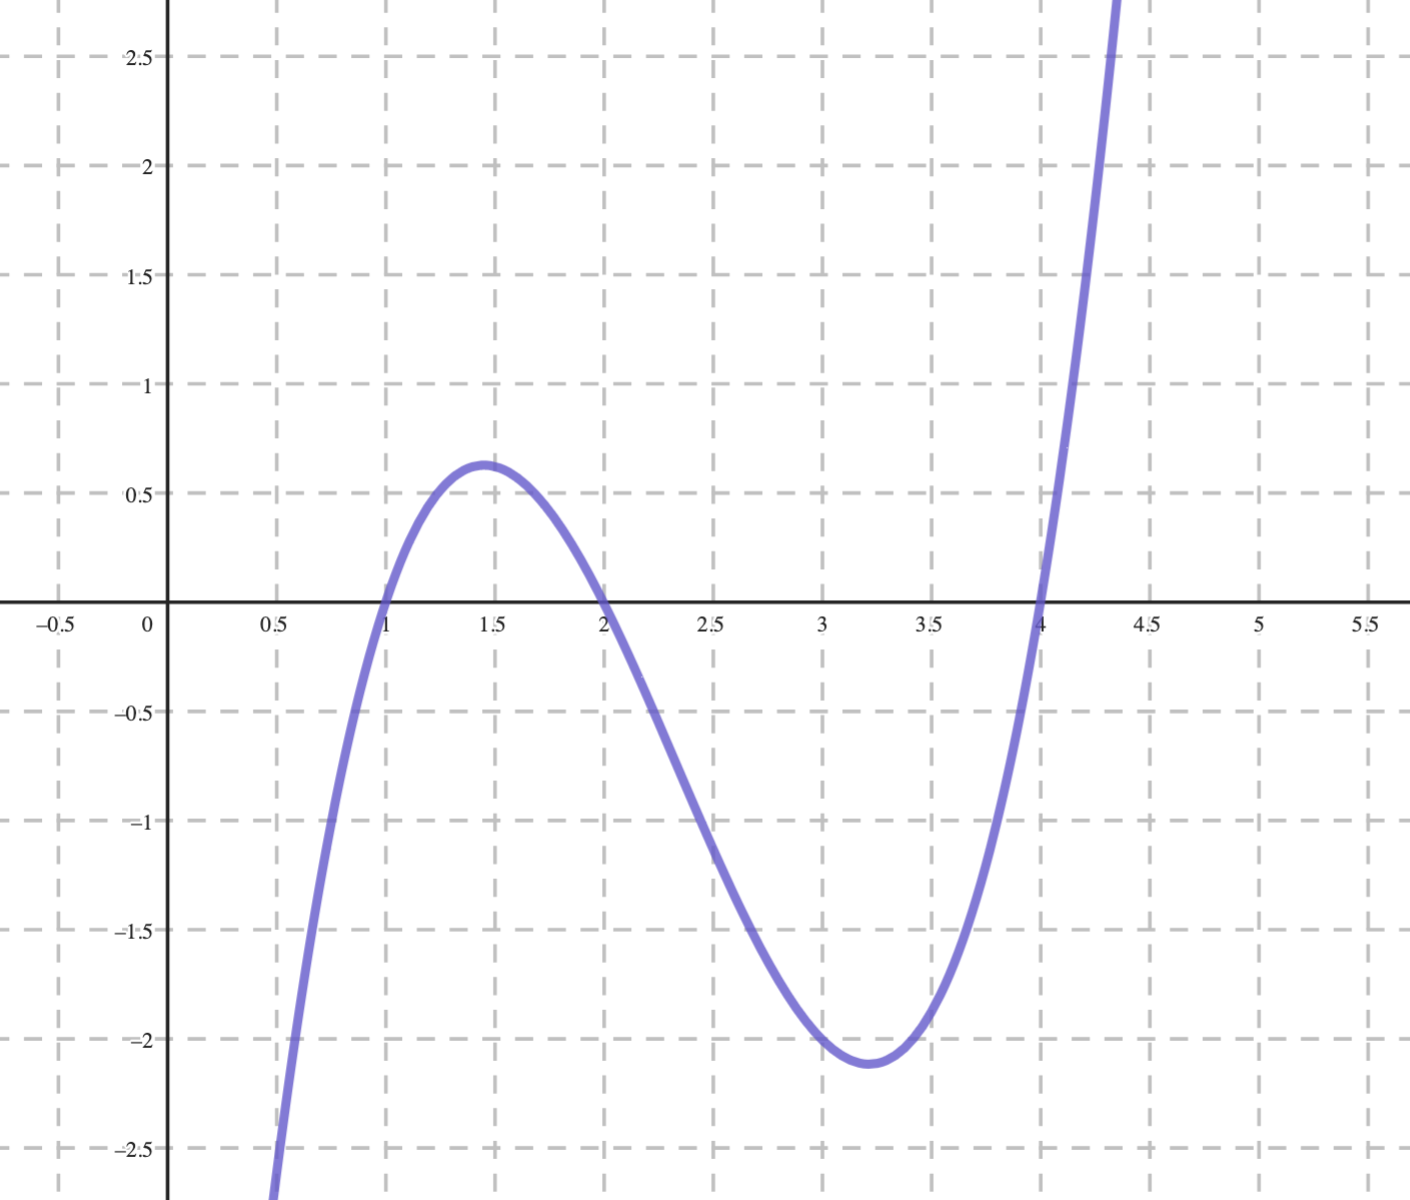
\includegraphics[width=0.7\textwidth]{images/lecture_13/vanishing.png}
            \caption{Vanishing polynomial $p(x)=(x-1)(x-2)(x-4)$ of $D=\{1,2,4\}$}
        \end{figure}
    \end{frame}

    \begin{frame}{Barycentric Interpolation}
        Now, let us come back to the interpolation problem $p(x_j) = a_j$ for $j \in [N]$.
        Introduce $\gamma(x) = \prod_{j=0}^{N-1}(x-x_j)$. 

        \begin{block}{Proposition}
            The Lagrange basis polynomial $\ell_j$ can be rewritten as:
            \begin{equation*}
                \ell_j(x) = \gamma(x) \cdot \frac{w_j}{x-x_j}, \quad w_j = \frac{1}{\sum_{k=0,k\neq j}^{N-1}(x_j-x_k)}.
            \end{equation*}
        \end{block}

        Let us substitute it into the interpolation formula:
        \begin{equation*}
            p(x) = \sum_{j=0}^{N-1}a_j\ell_j(x) = \sum_{j=0}^{N-1}a_j\gamma(x)\frac{w_j}{x-x_j} = \gamma(x)\sum_{j=0}^{N-1}\frac{w_j}{x-x_j}a_j.
        \end{equation*}
    \end{frame}

    \begin{frame}{Barycentric Interpolation (Cont.)}
        \begin{equation*}
            \boxed{\textbf{Barycentric Formula:} \; \; p(x) = \gamma(x)\sum_{j=0}^{N-1}\frac{w_j}{x-x_j}a_j}
        \end{equation*}

        \begin{alertblock}{Proposition}
            \begin{itemize}
                \item Computing $\{w_j\}_{j \in [N]}$ costs $\mathcal{O}(N^2)$
                operations \emph{before evaluation}.
                \item Both $\gamma(x)$ and sum requires $\mathcal{O}(N)$ operations.
            \end{itemize}
        \end{alertblock}

        But what happens if instead of $x_j$, we use $\omega^j \in \Omega_N$?
        \begin{equation*}
            \boxed{p(x) = \frac{x^N-1}{N}\sum_{j \in [N]}\frac{\omega^j}{x-\omega^j}a_j}
        \end{equation*}

        \textcolor{purple}{\textbf{Takeaway:}} We can interpolate in $\mathcal{O}(N)$ operations.
    \end{frame}

    \section{Number Theoretic Transform}

    \subsection{Three Gadgets}
    \begin{frame}{What is NTT?}
        Now suppose we want to find $m(x) = p(x)q(x)$. We'll use NTT!
        
        \begin{alertblock}{Question}
            What does it mean that you \emph{know} polynomial $p(x) \in \mathbb{F}^{(\leq N)}[x]$?
        \end{alertblock}

        This means either of two (typically):
        \begin{itemize}
            \item You know the polynomial coefficients $p_0,\dots,p_{N-1}$.
            \item You know the polynomial values at some points $\{(x_j,a_j)\}_{j \in [N]}$.
        \end{itemize}

        \begin{definition}[NTT]
            Suppose $p(x) = \sum_{j=0}^{N-1}p_jx^j$. The \textbf{Number Theoretic Transform} (NTT) of $p$ is defined as evaluations of $p$ at the $N$-th roots of unity:
            \begin{equation*}
                \mathsf{NTT}(p) = \left(p(\omega^0), p(\omega^1), \dots, p(\omega^{N-1})\right).
            \end{equation*}
        \end{definition}
    \end{frame}

    \begin{frame}{What is the point of NTT?}
        \textcolor{green!60!black}{\textbf{Note:}} To denote the result of NTT, we use hat: $\hat{p} = \mathsf{NTT}(p)$.

        \textcolor{purple}{\textbf{Question:}} Given NTTs $\hat{p}$ and $\hat{q}$ of two polynomials $p$ and $q$, 
        how do we find the NTT of their product $m(x) = p(x)q(x)$?

        \begin{block}{Main NTT Property}
            Suppose $m(x) = p(x)q(x)$ is the product of $p$ and $q$. Then,
            \begin{equation*}
                \hat{\boldsymbol{m}} = \hat{\boldsymbol{p}} \odot \hat{\boldsymbol{q}}
            \end{equation*}
        
            Speaking more formally, $\mathsf{NTT}: (\mathbb{F}^{(\leq N)}[X],\times) \to (\mathbb{F}^N, \odot)$ is 
            a homomorphism between a set of polynomials of degree up to $N$ and their NTT domain. With certain 
            appropriate technicalities, $\mathsf{NTT}$ can be extended to the isomorphism (namely, use $\mathbb{F}[X] / (X^N-1)$).
        \end{block}

        \textcolor{blue!60!black}{\textbf{Why?}} Well... $m(\omega^j)=p(\omega^j)q(\omega^j)$ \hspace{20px} \textbf{:/}
    \end{frame}

    \begin{frame}{Final Ingredient: Inverse NTT}
        Now, can we restore the polynomial $m(x)$ from its NTT $\hat{m}$? Of course!

        \begin{definition}{Inverse NTT}
            The \textbf{Inverse Number Theoretic Transform} (INTT) is a function 
            that restores the polynomial $m(x)$ from its evaluations $\hat{m}$:
            \begin{equation*}
                \mathsf{INTT}(\hat{m}) = (m_0,m_1,\dots,m_{N-1})
            \end{equation*}
        \end{definition}

        In its essence, we solve the interpolation problem:
        \begin{equation*}
            m(\omega^j) = \hat{m}_j, \quad j \in [N], \quad \text{\textbf{Goal}: find coefficients $m_0,\dots,m_{N-1}$}
        \end{equation*}
    \end{frame}

    \subsection{Polynomial vs NTT Domain}

    \begin{frame}{Punchline}
        \begin{figure}[H]
            \centering
            \begin{tikzpicture}[node distance=2.5cm, >=Stealth]
                % Zones
                \node[very thick, draw=blue, fill=blue, fill opacity=0.1,minimum width=9.5cm, minimum height=1.75cm,dashed,on background layer](targetbox) at (2.25, 0.1) {};
                \node(targetzonelabel)[above=0.65cm of targetbox,anchor=north,color=blue!90!black]{\textbf{Polynomial Space $\mathbb{F}^{(\leq N)}[x]$}};
            
                \node[very thick, draw=green, fill=green!80!black, fill opacity=0.1,minimum width=9.5cm, minimum height=2.0cm,dashed,on background layer](targetbox) at (2.25, -2.0) {};
                \node(targetzonelabel)[below=0.15cm of targetbox,anchor=north,color=green!60!black]{\textbf{NTT Space}};
            
                % Nodes
                \node (pq) at (0,0) {\( p, q \)};
                \node (m) [right=3cm of pq] {\( m = p \cdot q \)};
                \node (pHatqHat) [below=2cm of pq] {\( \hat{p}, \hat{q} \)};
                \node (mHat) [below=2cm of m] {\( \hat{m} = \hat{p} \odot \hat{q} \)};
                
                % Arrows
                \draw[->, line width = 0.5mm] (pq) -- (m) node[midway, above] {$\mathcal{O}(N^2)$};
                \draw[->, dashed, line width = 0.5mm] (pq) -- (pHatqHat) node[midway, left] {$\mathcal{O}(N \log N)$};
                \draw[->, dashed, line width = 0.5mm] (pHatqHat) -- (mHat) node[midway, above] {$\mathcal{O}(N)$};
                \draw[->, dashed, line width = 0.5mm] (mHat) -- (m) node[midway, right] {$\mathcal{O}(N \log N)$};
            
                % Labels
                \node at ($(pq)!0.5!(pHatqHat)$) [left] {};
                
                \end{tikzpicture}
            \caption{Illustration of the NTT Algorithm}
            \label{fig:ntt}
        \end{figure}

        \begin{alertblock}{Question}
            Does it resemble you one trick from Elliptic Curves?
        \end{alertblock}
    \end{frame}

    \begin{frame}{Illustration}
        \begin{figure}
            \centering
            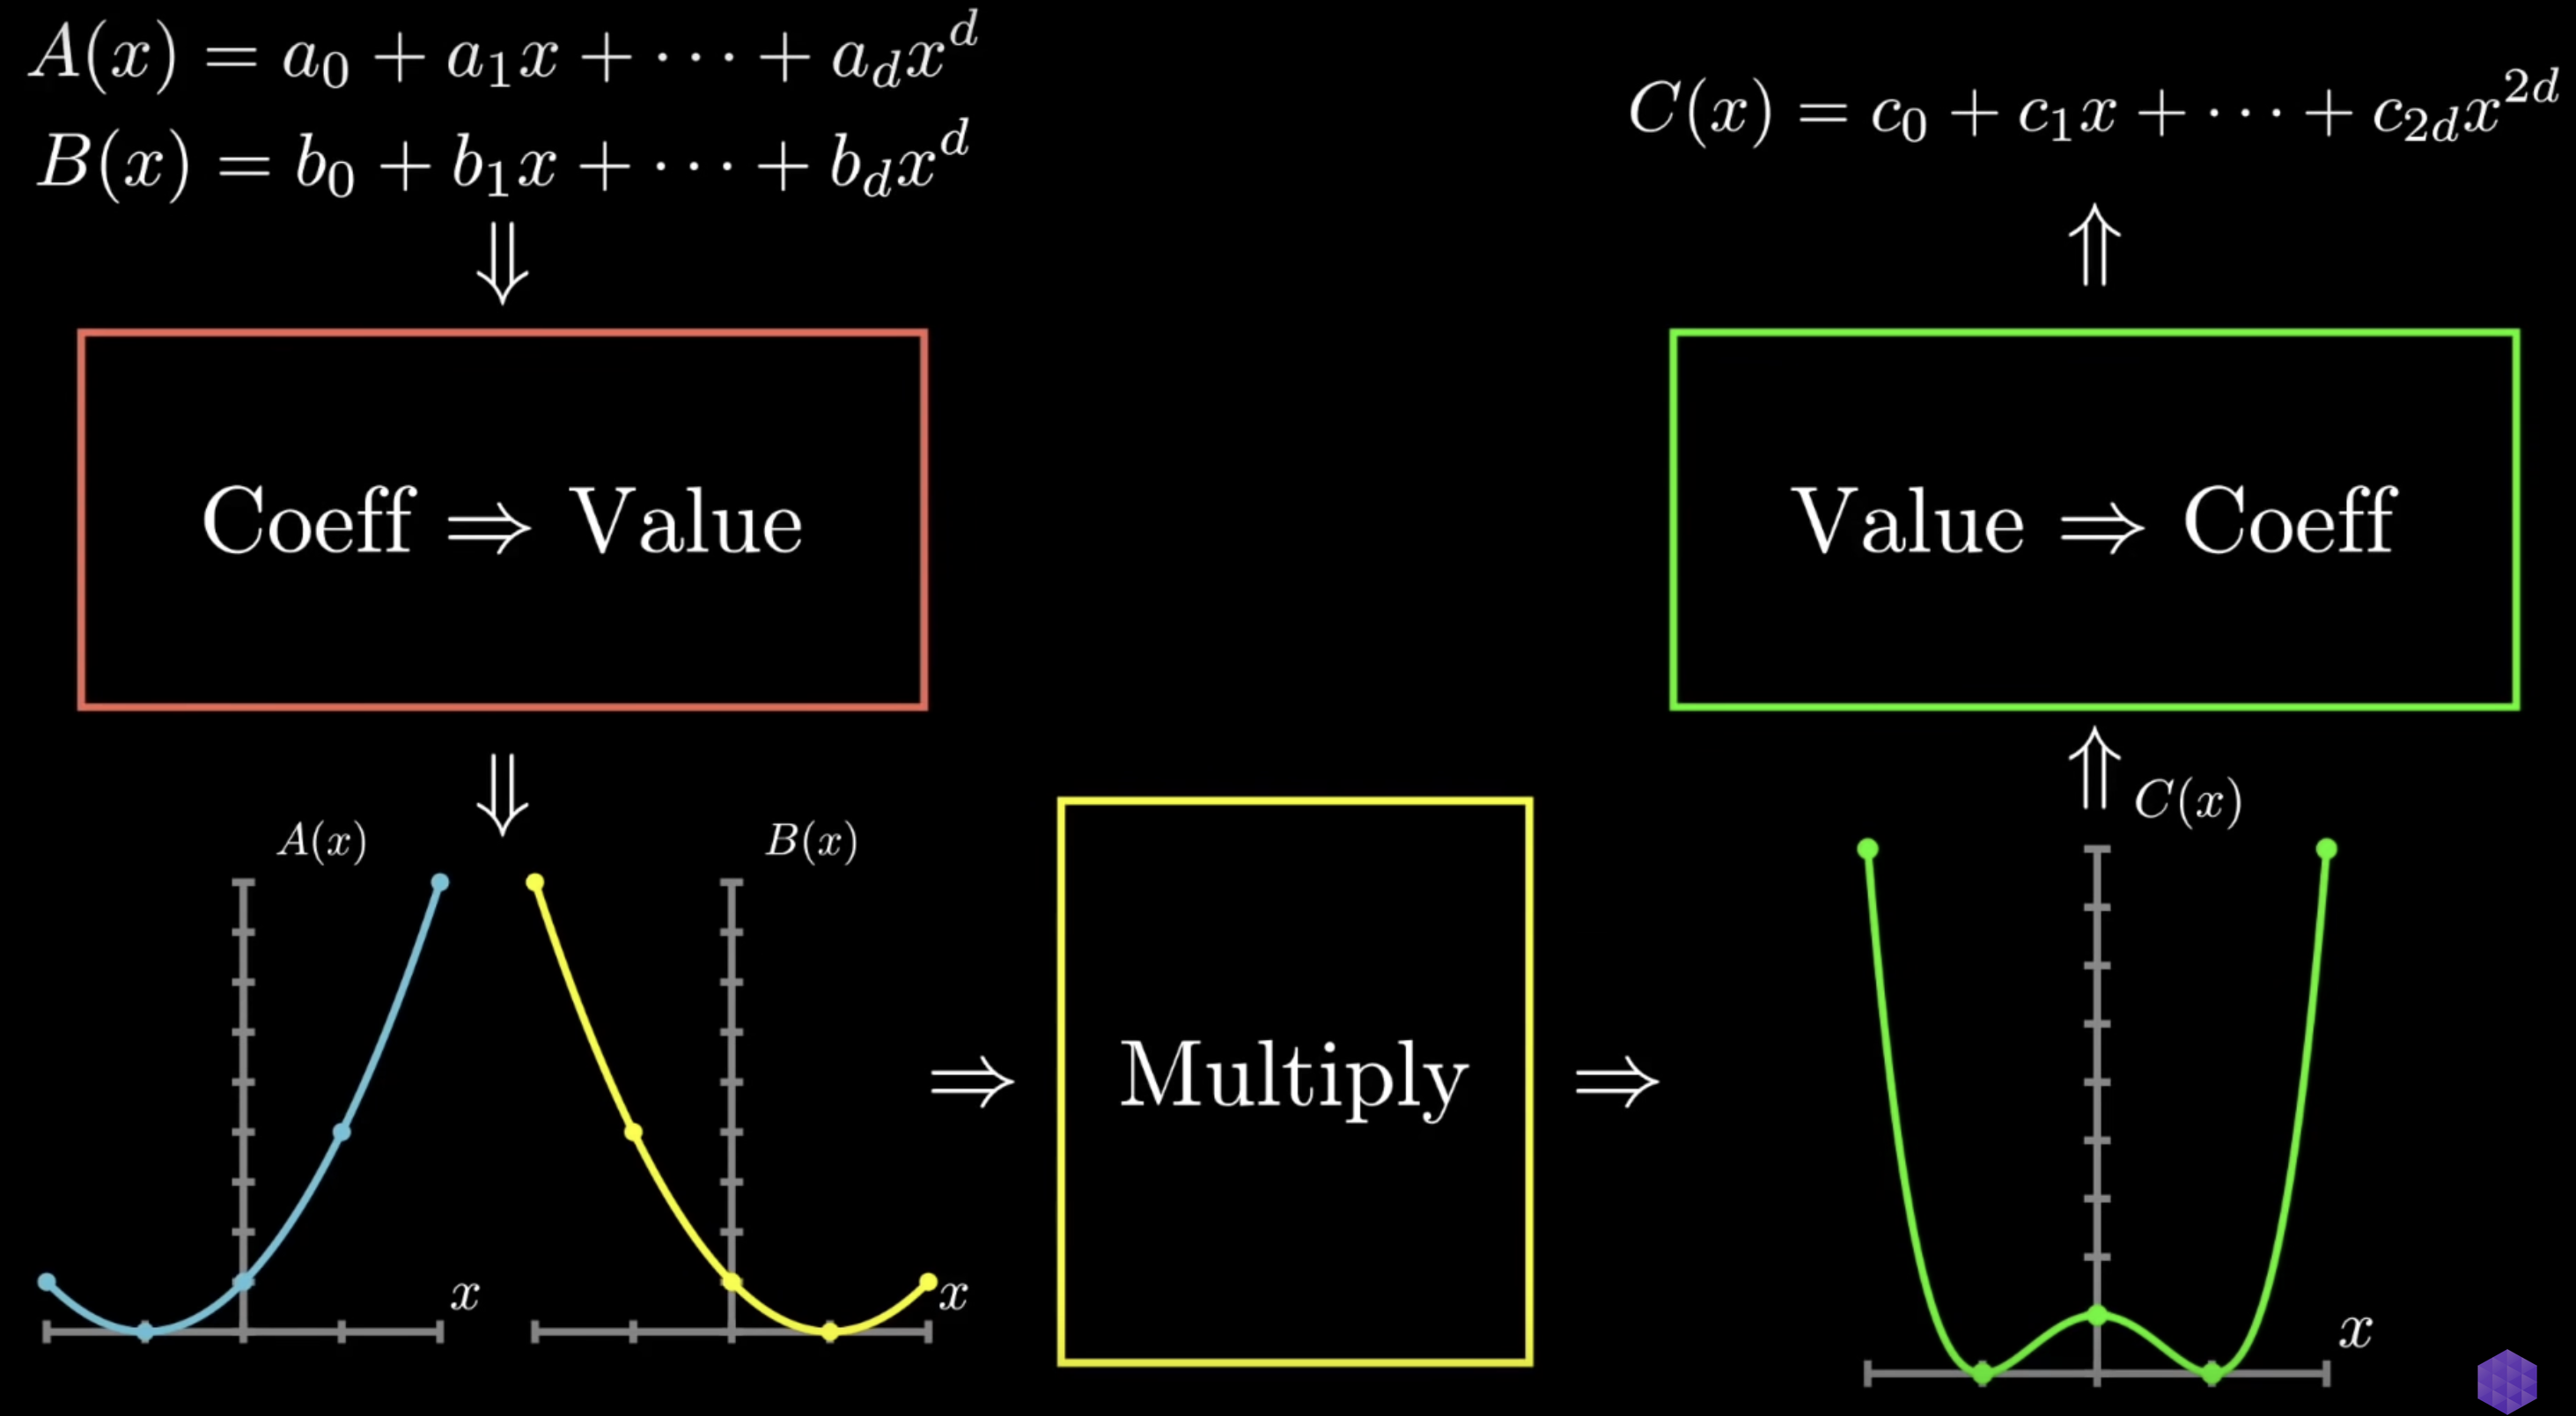
\includegraphics[width=\textwidth]{images/lecture_13/ntt_visualization.png}
            \caption{Illustration of the FFT Algorithm. Taken from ``The Fast Fourier Transform (FFT): Most Ingenious Algorithm Ever?''}
        \end{figure}
    \end{frame}

    \section{Details}

    \begin{frame}{When NTT works?}
        \begin{block}{Note}
            For NTT to work, we will impose the following requirements on 
            our setup:
            \begin{enumerate}
                \item The field $\mathbb{F}_p$ should have $2^k$-roots of unity for sufficiently many $k$. In other words, $p=p' \cdot 2^m + 1$ with \emph{small} $p' \in \mathbb{N}$.
                \item The polynomial order is $N=2^k$. Not a strict requirement, since we can always pad the polynomial with zeros.
            \end{enumerate}
        \end{block}

        \begin{example}
            \begin{itemize}
                \item \textbf{BabyBear prime} $p=15 \cdot 2^{27} + 1$ is NTT-friendly: the order of multiplicative
                group is $15 \cdot 2^{27}$, so $2^k \mid 15 \cdot 2^{27}$ for all $k \leq 27$.
                \item \textbf{Mersenne prime} $p=2^{31}-1$ is not NTT-friendly: the order of multiplicative 
                group is $2^{31}-2 = 2 \times (2^{30}-1)$.
            \end{itemize}
        \end{example}
    \end{frame}

    \subsection{Why NTT takes quasilinear complexity?}

    \begin{frame}{Why NTT takes quasilinear complexity?}
        Recall that we need to evaluate $N$ expressions:
        \begin{equation*}
            p(\omega^j) = \sum_{i=0}^{N-1}p_i(\omega^j)^i = \sum_{i=0}^{N-1}p_i\omega^{ij}, \quad j \in [N].
        \end{equation*}

        \textcolor{purple}{\textbf{Naive Complexity:}} $\mathcal{O}(N^2)$ operations. We need $N$ evaluations, 
        each of which requires $N$ multiplications.

        \begin{align*}
            p(\omega^j) &= \sum_{i=0}^{2^r-1}p_i\omega^{ij} = \sum_{i=0}^{2^{r-1}-1}p_{2i}\omega^{2ij} + \sum_{i=0}^{2^{r-1}-1}p_{2i+1}\omega^{j(2i+1)}\\
            &= \textcolor{green!60!black}{\sum_{i=0}^{2^{r-1}-1}p_{2i}(\omega^{2j})^i} + \omega^j\textcolor{blue!60!black}{\sum_{i=0}^{2^{r-1}-1}p_{2i+1}(\omega^{2j})^i}.
        \end{align*}
    \end{frame}

    \begin{frame}{Folding}
        Denote $p_E(x) = \sum_{i=0}^{2^{r-1}-1}p_{2i}x^i$ and $p_O(x) = \sum_{i=0}^{2^{r-1}-1}p_{2i+1}x^i$. Then,
        \begin{equation*}
            p(\omega^j) = \textcolor{green!60!black}{p_E(\omega^{2j})} + \omega^j \textcolor{blue!60!black}{p_O(\omega^{2j})}.
        \end{equation*}

        \begin{block}{Fact \#1}
            We need only $N/2$ evaluations from $\Omega$ of $p_E$ and $p_O$. Note that:
            \begin{equation*}
                p(\omega^{j+N/2}) = \textcolor{green!60!black}{p_E(\omega^{2j})} + \omega^j\omega^{N/2} \textcolor{blue!60!black}{p_O(\omega^{2j})}.
            \end{equation*}
        \end{block}

        \begin{block}{Fact \#2}
            \begin{itemize}
                \item We need to evaluate two $N/2$-degree polynomials.
                \item We need to evaluate them at $N/2$ points.
            \end{itemize}

            Thus, we shrink the problem size by half at each step.
        \end{block}
    \end{frame}

    \begin{frame}{Algorithm Summarized}
        \begin{algorithm}[H]
            \caption{Number Theoretic Transform (NTT)}
            \Input{Polynomial $p(x) = \sum_{j=0}^{N-1}p_jx^j$}
            \Output{Vector of evaluations $\mathsf{NTT}(\boldsymbol{p}, \omega)$ at $\Omega=\{\omega\}_{j \in [N]}$}
        
            \If{$N=1$}{
                \Return{$(p_0)$}
            }
        
            $H \gets N/2$ \Comment{Compute the domain half-size}
        
            $\boldsymbol{p}_{E} \gets (p_0,p_2,\dots,p_{N-2})$ \Comment{Find even-indexed coefficients}
        
            $\boldsymbol{p}_{O} \gets (p_1,p_3,\dots,p_{N-1})$ \Comment{Find odd-indexed coefficients}
        
            $\boldsymbol{y}_E \gets \mathsf{NTT}(\boldsymbol{p}_{E}, \omega^2)$ \Comment{Compute NTT for even polynomial via $\frac{N}{2}$th primitive root $\omega^2$}
        
            $\boldsymbol{y}_O \gets \mathsf{NTT}(\boldsymbol{p}_O, \omega^2)$ \Comment{Compute NTT for odd polynomial via $\frac{N}{2}$th primitive root $\omega^2$}
        
            \Return{$(y_0,\dots,y_{N-1})$ with $y_j=y_{E, \;j \; \text{mod} \; H} + \omega^j y_{O, \; j \; \text{mod} \; H}$}
        \end{algorithm}
    \end{frame}

    \begin{frame}{Inverse NTT}
        \begin{theorem}
            The Inverse NTT can be computed in the same way as NTT, but with the 
            inverse primitive root $\omega^{-1}$:
            \begin{equation*}
                p_j = \frac{1}{N}\sum_{i=0}^{N-1}\omega^{-ij}\hat{p}_i
            \end{equation*}

            Thus, its complexity is also $\mathcal{O}(N \log N)$.
        \end{theorem}

        \begin{block}{Conclusion}
            To compute $m(x) = p(x)q(x)$, simply use the following:
            \begin{equation*}
                m(x) = \mathsf{INTT}(\mathsf{NTT}(p) \odot \mathsf{NTT}(q))
            \end{equation*}

            The total complexity remains $\mathcal{O}(N \log N)$.
        \end{block}
    \end{frame}

    \begin{frame}[plain, standout]
        \centering
        \LARGE
        \textbf{Thank you for your attention} \\

        \vspace{0.2cm} \Huge \ding{170} \large \\

        \vspace{1cm}

        \href{https://zkdl-camp.github.io/}{\raisebox{-.1em}{\hspace{.025em}\faIcon{globe}}\hspace{.325em}zkdl-camp.github.io} \\

        \href{https://github.com/ZKDL-Camp}{\raisebox{-.1em}{\hspace{.025em}\faIcon{github}}\hspace{.325em}github.com/ZKDL-Camp}

        \begin{center}
            
\includegraphics[width=0.15\textwidth]{images/logo.png}
        \end{center}
    \end{frame}
\end{document}